\documentclass[12pt,a4paper]{article}
\usepackage{amsmath, amssymb}
\usepackage{array}
\usepackage{tikz}

\title{MATH1064 Assignment1}
\author{SID:530157791}
\date{\today}

\begin{document}

\maketitle


\subsection*{Answer to question1}
1.$p \rightarrow q$\qquad\qquad(Premise)\\
2.$(r \lor s) \rightarrow (p \land \neg q)$\qquad\qquad(Premise)\\
3.$\neg p \lor q$\qquad\qquad(conditional to disjunction from 1)\\
4.$\neg (r \lor s) \lor (p \land \neg q)$\qquad\qquad(conditional to disjunction from 2)\\
5.$\neg \neg (\neg p \lor q)$\qquad\qquad(double negative from 3)\\
6.$\neg (p \land \neg q)$\qquad\qquad(De Morgan’s laws from 5)\\
7.$\neg (r \lor s)$\qquad\qquad(Disjunctive Syllogism from 4\&6)\\
8.$\neg r \land \neg s$\qquad\qquad(De Morgan’s laws from 7)\\
9.$\neg r$\qquad\qquad(specialisation from 8)\\


==================================================================================================
\newpage
==================================================================================================

\subsection*{answer to question2}

\begin{table}[h]
\centering
\begin{tabular}{|c|c|c|c|c|c|c|c|c|c|}
\hline
\( p \) & \( q \) & \( r \) & \( \neg q \) & \( \neg r \) & \( p \land \neg q \)&\( p \land \neg q \land \neg r \) & \(p \lor q\)& \( \neg (p \lor q) \) & \( (p \land \neg q \land \neg r) \lor \neg (p \lor q) \) \\
\hline
T & T & T & F & F & F & F & T& F & F \\
T & T & F & F & T & F & F & T& F & F \\
T & F & T & T & F & T & F & T& F & F \\
T & F & F & T & T & T & T & T& F & T \\
F & T & T & F & F & F & F & T& F & F \\
F & T & F & F & T & F & F & T& F & F \\
F & F & T & T & F & F & F & F& T & T \\
F & F & F & T & T &  F & F & F& T & T \\
\hline
\end{tabular}
\caption{Truth table for first proposition}
\end{table}


\begin{table}[h]
\centering
\begin{tabular}{|c|c|c|c|c|c|c|c|}
\hline
\( p \) & \( q \) & \( r \) & \( \neg q \) & \( p \land \neg q \) & \( \neg (p \land \neg q) \) & \( r \rightarrow \neg (p \land \neg q) \) & \( (r \rightarrow \neg (p \land \neg q)) \land \neg q \) \\
\hline
T & T & T & F & F & T & T & F \\
\hline
T & T & F & F & F & T & T & F \\
\hline
T & F & T & T & T & F & F & F \\
\hline
T & F & F & T & T & F & T & T \\
\hline
F & T & T & F & F & T & T & F \\
\hline
F & T & F & F & F & T & T & F \\
\hline
F & F & T & T & F & T & T & T \\
\hline
F & F & F & T & F & T & T & T \\
\hline
\end{tabular}
\caption{Truth table for second proposition}
\end{table}


==================================================================================================
\newpage
==================================================================================================

Simplify truth tables\\

\begin{table}[h]
    \centering
    \begin{minipage}{0.45\textwidth}
        \centering
        \begin{tabular}{|c|c|c|c|}
            \hline
            \( p \) & \( q \) & \( r \) & \( (p \land \neg q \land \neg r) \lor \neg (p \lor q) \) \\
            \hline
            T & T & T & F \\
            T & T & F & F \\
            T & F & T & F \\
            T & F & F & T \\
            F & T & T & F \\
            F & T & F & F \\
            F & F & T & T \\
            F & F & F & T \\
            \hline
        \end{tabular}
        \caption{simple truth table for first proposition, only contains proposition and p,q,r}
    \end{minipage}
    \hfill
    \begin{minipage}{0.45\textwidth}
        \centering
        \begin{tabular}{|c|c|c|c|}
            \hline
            \( p \) & \( q \) & \( r \) & \( (r \rightarrow \neg(p \land \neg q)) \land \neg q \) \\
            \hline
            T & T & T & F \\
            T & T & F & F \\
            T & F & T & F \\
            T & F & F & T \\
            F & T & T & F \\
            F & T & F & F \\
            F & F & T & T \\
            F & F & F & T \\
            \hline
        \end{tabular}
        \caption{simple truth table for second proposition, only contains proposition and p,q,r}
    \end{minipage}
\end{table}

From the truth table, it's evident that the two compound propositions are logically equivalent as they have the same truth values for all possible combinations of p, q, and r.

==================================================================================================
\newpage
==================================================================================================

\subsection*{answer to question3}

(a) \textbf{True}\\
There are 2 possibilities:\\\\
case1  :  If $k \geq 0$, then $Q(k)$ is true by defintion because $k$ is a non-negative number. Thus,  $Q(k) \lor Q(-k)$ is true since $Q(k)$ is true when $k \geq 0$.\\\\
case2  :  If $k < 0$,then $-k \geq 0$ ,then $Q(-k)$ is true by defintion.Thus,  $Q(k) \lor Q(-k)$ is true since $Q(-k)$ is true when $k < 0$.\\\\
Therefore, $\forall k \in \mathbb{Z},Q(k) \lor Q(-k)$ is true.\\\\
The negation of this statement is $\exists k \in \mathbb{Z},\neg Q(k) \land \neg Q(-k)$.\\\\\\
(b) \textbf{True}\\
There are 3 possibilities:\\\\
case1  :  If $k1 \geq 0 ,  k2 \geq 0$, then $Q(k1) \land Q(k2)$ is true by defintion.\\
In this case, $k1 * k2 \geq 0$ because $k1$ and $k2$ are none-negative integers ,  then $Q(k1 * k2)$ is true by definition.$Q(k1) \land Q(k2)$ and $Q(k1 * k2)$ are true in this case. Thus ,  $Q(k1) \land Q(k2) \rightarrow Q(k1 * k2)$ is true when $k1 \geq 0 ,  k2 \geq 0$.\\\\
case2 : If $k1 < 0,k2 < 0$, then $Q(k1) \land Q(k2)$ is false because $k1,k2$ are not non-negative integers. In this case , whether $Q(k1 * k2)$ is true or not,  $Q(k1) \land Q(k2) \rightarrow Q(k1 * k2)$ must be true. Thus ,  $Q(k1) \land Q(k2) \rightarrow Q(k1 * k2)$ is true when $k1 < 0 ,  k2 < 0$.\\\\
case3 : If $k1 < 0$ or $k2 < 0$ , then $Q(k1)$ or $Q(k2)$ is false by definition . Then $Q(k1) \land Q(k2)$ is false. In this case , whether $Q(k1 * k2)$ is true or not,  $Q(k1) \land Q(k2) \rightarrow Q(k1 * k2)$ must be true. Thus ,  $Q(k1) \land Q(k2) \rightarrow Q(k1 * k2)$ is true when $k1 < 0 ,  k2 < 0$.\\\\
Therefore ,$\forall k1,k2 \in \mathbb{Z}$,$Q(k1) \land Q(k2) \rightarrow Q(k1 * k2)$ is true.

==================================================================================================
\newpage
==================================================================================================
\\\\
(c) \textbf{False}\\
There are 3 possibilities:\\\\
case1  :  If $k1 \geq 0 ,  k2 \geq 0$, then $k1 * k2 \geq 0$ , $Q(k1 * k2)$ is true by defintion.$Q(k1) \land Q(k2)$ is also true. Thus,  $Q(k1 * k2) \rightarrow Q(k1) \land Q(k2)$ is true when $k1 \geq 0 ,  k2 \geq 0$.\\\\
case2 : If $k1 < 0 ,  k2 < 0$, then $k1 * k2 > 0$ , $Q(k1 * k2)$ is true by defintion.$Q(k1) \land Q(k2)$ is false because $k1$ and $k2$ are not none-negative integers.Thus,  $Q(k1 * k2) \rightarrow Q(k1) \land Q(k2)$ is false when $k1 < 0$and$ k2 < 0$.\\\\
case3 : If $k1 < 0$ or $k2 < 0$ , Then $k1 * k2 < 0$,Q(k1 * k2) is false. Thus $Q(k1 * k2) \rightarrow Q(k1) \land Q(k2)$ is true when $k1 < 0$ or $k2 < 0$.\\\\
Therefore ,$\forall k1,k2 \in \mathbb{Z},Q(k1 * k2) \rightarrow Q(k1) \land Q(k2)$ is false due to $Q(k1 * k2) \rightarrow Q(k1) \land Q(k2)$ is false when $k1 < 0 ,  k2 < 0$\\\\\\
(d) \textbf{True}\\
There are 2 possibilities:\\\\
case1 : If $k1$ is even and $k2$ is divisible by 3,then $R(k1) \land R(k2)$ is true. Let $k1 = 2m,m \in \mathbb{Z},k2 = 3n, n \in \mathbb{Z}$.Then $3k1 + 2k2$ can be written as $2 * 3 * (m + n)$.So that $3k1 + 2k2$ is a even number and also divisible by 3.Then 
$R(3k1 + 2k2) \land Q(3k1 + 2k2)$ is true.Thus ,  $R(k1) \land R(k2) \rightarrow R(3k1 +2k2) \land S(3k1 + 2k2)$ is true. \\\\
case2 : If k1 is not even or k2 is not  divisible by 3 , or k1 is not even and k2 is not divisible by 3.Then $R(k1) \land R(k2)$ must be flase. Thus ,$R(k1) \land R(k2) \rightarrow R(3k1 +2k2) \land S(3k1 + 2k2)$ is true. \\\\
Therefore, $\forall k1 , k2 \in \mathbb{Z},R(k1) \land R(k2) \rightarrow R(3k1 +2k2) \land S(3k1 + 2k2)$ is true. \\\\

==================================================================================================
\newpage
==================================================================================================
\\
(e) \textbf{True}\\
There are 4 possibilities:\\\\
case1 : If $k1$ is even and $k2$ is divisible by 3,then $R(k1) \lor S(k2)$ is true. Let $k1 = 2m,m \in \mathbb{Z},k2 = 3n, n \in \mathbb{Z}$.Then $3k1 + 2k2$ can be written as $2 * 3 * (m + n)$.So that $3k1 + 2k2$ is a even number and also divisible by 3.Then 
$R(3k1 + 2k2) \lor Q(3k1 + 2k2)$ is true.Thus ,  $R(k1) \lor S(k2) \rightarrow R(3k1 +2k2) \lor S(3k1 + 2k2)$ is true. \\\\
case2 : If $k1$ is even but $k2$ is not divisible by 3,then $R(k1) \lor S(k2)$ is true.  Let $k1 = 2n , n \in \mathbb{Z}$,
then $3k1 + 2k2$ can be written as $2*(3n + k2)$,which is a even number.Then $R(3k1 + 2k2)$ is  true by definition.Such that $R(3k1 + 2k2) \lor S(3k1 +2k2)$ is true.Thus ,  $R(k1) \lor S(k2) \rightarrow R(3k1 +2k2) \lor S(3k1 + 2k2)$ is true. \\\\
case3 : If $k1$ is not even but $k2$ is divisible by 3,then $R(k1) \lor S(k2)$ is true.  Let $k2 = 3n , n \in \mathbb{Z}$,
then $3k1 + 2k2$ can be written as $3(k1 + 2n)$,which is divisible by 3.Then $S(3k1 + 2k2)$ is  true by definition.Such that $R(3k1 + 2k2) \lor S(3k1 +2k2)$ is true.Thus ,  $R(k1) \lor S(k2) \rightarrow R(3k1 +2k2) \lor S(3k1 + 2k2)$ is true. \\\\
case 4 : If $k1$ is not even and $k2$ is not divisible by 3,then $R(k1) \lor S(k2)$ is false. Then whether
$R(3k1 + 2k2) \lor Q(3k1 + 2k2)$ is true or not  , $R(k1) \lor S(k2) \rightarrow R(3k1 +2k2) \lor S(3k1 + 2k2)$ is true. \\\\\\
(f) \textbf{False}\\
case 1 : If k1 is even,then $\neg R(k1)$ is false. This statement is false.\\\\
case 2 : If k1 is odd ,then $\neg R(k1)$ is true. But $3k1 + 2k2$ is odd ,such that $R(3k1 + 2k2)$ is false ,this statment is false.\\
Negation : $\forall k1,k2 \in \mathbb{Z},\neg R(3k1 + 2k2) \lor R(k1)$



==================================================================================================
\newpage
==================================================================================================
\\
(g) \textbf{false}\\
Let $k = 6m,m \in \mathbb{N}$,then k is a even number and is divisible by 3.So that $R(k) \land S(k)$ is true.Assume that $l = 12m$,$\neg (R(l) \land S(l))$ is false.\\
Therefore , this statement is false.\\\\

\subsection*{answer to question4}

\begin{center}
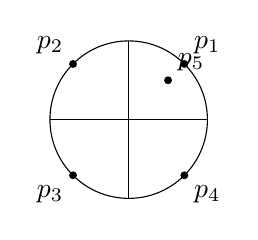
\begin{tikzpicture}
    % Draw the circle with radius 1
    \draw (0,0) circle (1);
    
    % Draw the diameters to split the circle into 4 quadrants
    \draw (-1,0) -- (1,0);
    \draw (0,-1) -- (0,1);
    
    % Label and place the 5 points on the circle (adjust as needed)
    \fill (0.707,0.707) circle (0.05) node[above right] {$p_1$};
    \fill (-0.707,0.707) circle (0.05) node[above left] {$p_2$};
    \fill (-0.707,-0.707) circle (0.05) node[below left] {$p_3$};
    \fill (0.707,-0.707) circle (0.05) node[below right] {$p_4$};
    \fill (0.5,0.5) circle (0.05) node[above right] {$p_5$}; % 将点p5移至圆内部。
\end{tikzpicture}
\end{center}

As illustrated in the figure, the circle is divided into 4 equal sectors. Assume that the 5 points are not located at the intersections of the sectors (this can be achieved by adjusting the direction of the divisions).\\Placing $ \{p1,p2,p3,p4,p5\}$ into these 4 sectors,at least one sector must contain 2 of these points by the pigeonhole principle.

The distance between 2 points in the same sector is smaller than $\sqrt2$(because the diameter splits the circle into these sectors).\\
Therefore, by pigeonhole principle,$\exists pj,pk \in \mathbb{P} : (j \neq k) \lor (d(pj,pk) < \sqrt2 )$ is true.


\end{document}
